\documentclass{article}

\usepackage[utf8]{inputenc}
\usepackage[T1]{fontenc}
\usepackage{a4wide}
\usepackage[french]{babel}
\usepackage[babel=true]{csquotes}
\usepackage{graphicx}
\graphicspath{{Images/}}
\usepackage{color}
\usepackage{hyperref}
% \hypersetup{colorlinks,linkcolor=,urlcolor=blue}

\usepackage{amsmath}
\usepackage{amssymb}


\title{Rapport de projet de développement d'une application mobile : Lotoquinote}
\author{David Boisedu et Alexandre Boyer}
\date{\today}

\begin{document}


\maketitle

\begin{abstract}
\begin{center}
L'application que nous avons développée répond à la problématique suivante : 
\newline \textit{Comment faciliter le suivi de tirage des numéros d'un loto quine grâce à une application mobile ?}
\end{center}
\end{abstract}

\section{Introduction}
\label{section:intro}

Cela peut être parfois fastidieux de noter sur une feuille tous les numéros sortis lors d'un tirage de loto-quine. C'est pour cette raison précise que nous avons décidé de créer une application qui faciliterai cette tâche. En plus de permettre de suivre le tirage d'un loto-quine, l'application Lotoquinote permet aussi d'enregistrer chaque tirage pour pouvoir les consulter à n'importe quel moment. De plus, grâce à des fonctions de tri, il est possible de voir très rapidement les numéros qui ont été tirés lors d'un tirage.

\section{Description générale de l'application}

L'application Lotoquinote comporte trois vues :

\begin{itemize}
\vspace{1em}
    \item {\underline {\large{La vue d'accueil :}}}
\end{itemize} 
    \noindent%
    \begin{minipage}{.6\textwidth}%
    Cette vue permet la création d'un nouveau suivi de tirage et affiche tous les suivis de tirage crées sous forme de liste pouvant être défilée. 
    \end{minipage}%
    \hfill
    \begin{minipage}{.35\textwidth}%
        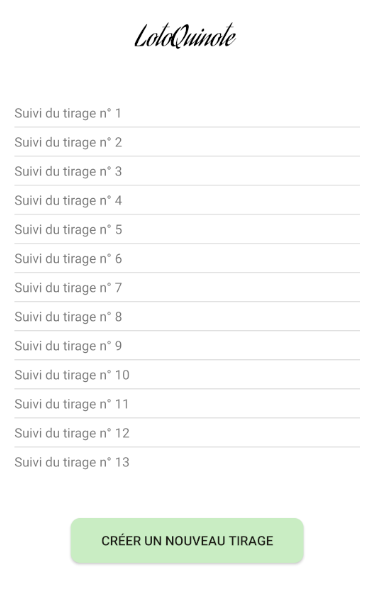
\includegraphics[scale=0.6]{accueil.png}
    \end{minipage}%
    
    \begin{minipage}{.35\textwidth}%
        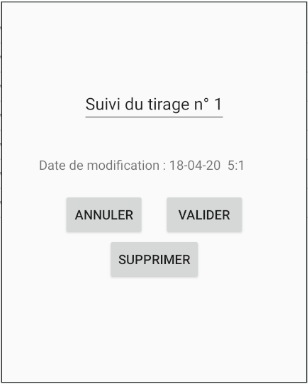
\includegraphics[scale=0.6]{edition.png}
    \end{minipage}%
    \hfill
    \begin{minipage}{.6\textwidth}%
    La vue d'accueil possède aussi une fonctionnalité d'édition lors d'un appui-long sur un suivi de tirage. Cette fonctionnalité permet de :
    \vspace{1em}
    \begin{itemize}
        \item Mofidier le titre du suivi de tirage
        \item Afficher la date de dernière modification
        \item Supprimer le suivi de tirage
    \end{itemize}
    \end{minipage}%
\vspace{4em}
\begin{itemize}
    \item {\underline{\large{La vue de suivi de tirage :}}}
\end{itemize}
\vspace{1em}
    \begin{minipage}{.6\textwidth}%
    La vue de suivi de tirage permet de choisir le numéro qui a été tiré lors du tirage du loto-quine. Le numéro est choisit soit par le biais du NumberPicker ou soit en l'écrivant soi-même grâce à l'EditText.
    \vspace{1em}
    \newline
    Lors du clique sur le bouton "Ajouter", le numéro choisit est inséré à la liste des numéros tirés. Les cinq derniers numéros tirés de cette liste sont visibles dans les cases situées en bas de cette vue.
    Le bouton "Terminer" permet de revenir à la vue d'accueil.
    \vspace{1em}
    \newline
    La croix située en-dessous de la 1ère case à gauche permet de supprimer le dernier numéro ajouté à la liste.
    \newline
    Le bouton "+" à droite de la dernière case permet de basculer sur la vue de la liste complète des numéros tirés. 
    \end{minipage}%
    \hfill
    \begin{minipage}{.35\textwidth}%
        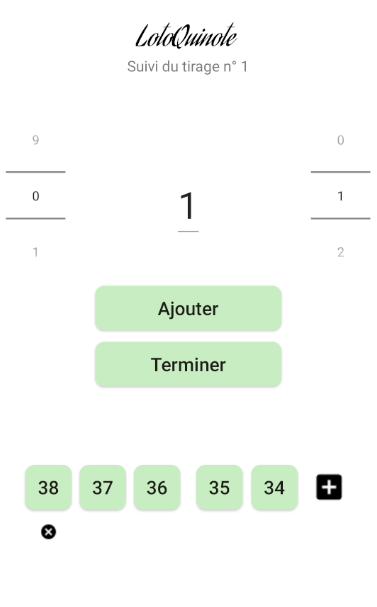
\includegraphics[scale=0.6]{suivi.png}
    \end{minipage}%
\vspace{2em}
\newline
\underline{Remarque :}  A chaque ajout d'un numéro à la liste, un toast nous informe que celui-ci a bien été ajouté. Si le numéro que l'on veut ajouter est déjà présent dans la liste un toast apparaît pour signaler le fait que ce numéro a déjà été tiré et qu'il ne sera donc pas ajouté.
\newpage
\begin{itemize}
    \item {\underline{\large{La vue de la liste des numéros tirés :}}}
\end{itemize}
\vspace{1em}
    \begin{minipage}{.35\textwidth}%
        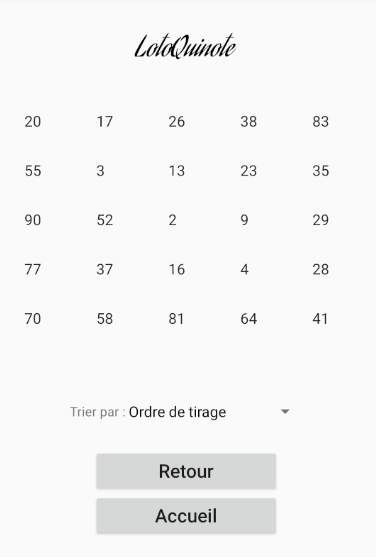
\includegraphics[scale=0.6]{liste.png}
    \end{minipage}%
    \hfill
    \begin{minipage}{.6\textwidth}%
    Cette vue permet de voir l'ensemble des numéros tirés lors du tirage du loto-quine. Par défaut, les numéros sont triés par ordre de tirage : le dernier numéro tiré est le premier de la liste.
    \vspace{1em}
    \newline
    D'autres fonctions de tri sont disponibles par le biais d'une petite liste déroulante. On peut ainsi trier les numéros par :
    \begin{itemize}
        \item Ordre de tirage
        \item Ordre croissant
        \item Ordre décroissant
    \end{itemize}
    \end{minipage}%
    
    
    


\section{Architecture du code}

\subsection{Android}

    \begin{minipage}{.6\textwidth}%
    Le code de notre application suit l'architecture MVC \newline (Modèle, Vue, Contrôleur).
    \vspace{1em}
    \newline Ainsi, la partie "Contrôleur" contient les activités principales de notre application.
    \vspace{1em}
    \newline La partie "Modèle" contient les classes que nous utilisons pour définir les objets nécessaires à notre application.
    \vspace{1em}
    \newline Et la partie "Vue" représenté par le dossier "layout" contient les fichiers .xml qui permettent l'interaction entre l'application et l'utilisateur. 
    \end{minipage}%
    \hfill
    \begin{minipage}{.35\textwidth}%
        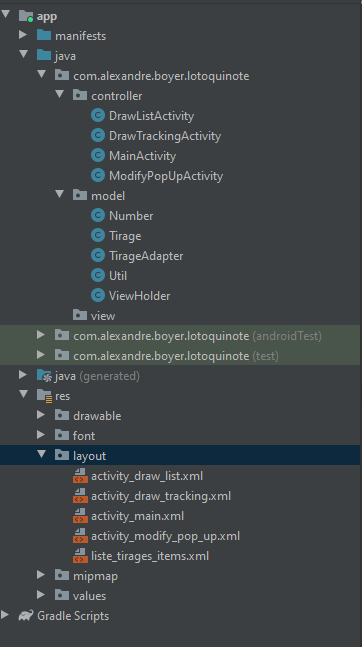
\includegraphics[scale=0.5]{archiMVC.png}
    \end{minipage}%

\section{Quelques points délicats/intéressants}

\section{Conclusion}

\begin{thebibliography}{}
\bibitem{}

\end{thebibliography}

\end{document}
